\documentclass[12pt]{article}
\usepackage[margin=1in]{geometry}
\usepackage{setspace}
\onehalfspacing

% Start of preamble
%==========================================================================================%
% Required to support mathematical unicode
\usepackage[warnunknown, fasterrors, mathletters]{ucs}
\usepackage[utf8x]{inputenc}

\usepackage[dvipsnames,table,xcdraw]{xcolor}

% Standard mathematical typesetting packages
\usepackage{amsmath,amssymb,amscd,amsthm,amsxtra, pxfonts}
\usepackage{mathtools,mathrsfs,dsfont,xparse}

% Symbol and utility packages
\usepackage{cancel, textcomp}
\usepackage[mathscr]{euscript}
\usepackage[nointegrals]{wasysym}
\usepackage{apacite}

% Extras
\usepackage{physics}  
\usepackage{tikz-cd} 
\usepackage{microtype}
\usepackage{enumitem}
\usepackage{titling}
\usepackage{graphicx}

% Fancy theorems due to @intuitively on discord
\usepackage{mdframed}
\newmdtheoremenv[
backgroundcolor=NavyBlue!30,
linewidth=2pt,
linecolor=NavyBlue,
topline=false,
bottomline=false,
rightline=false,
innertopmargin=10pt,
innerbottommargin=10pt,
innerrightmargin=10pt,
innerleftmargin=10pt,
skipabove=\baselineskip,
skipbelow=\baselineskip
]{mytheorem}{Theorem}

\newenvironment{theorem}{\begin{mytheorem}}{\end{mytheorem}}

\newtheorem{corollary}{Corollary}
\newtheorem{lemma}{Lemma}

\newtheoremstyle{definitionstyle}
{\topsep}%
{\topsep}%
{}%
{}%
{\bfseries}%
{.}%
{.5em}%
{}%
\theoremstyle{definitionstyle}
\newmdtheoremenv[
backgroundcolor=Violet!30,
linewidth=2pt,
linecolor=Violet,
topline=false,
bottomline=false,
rightline=false,
innertopmargin=10pt,
innerbottommargin=10pt,
innerrightmargin=10pt,
innerleftmargin=10pt,
skipabove=\baselineskip,
skipbelow=\baselineskip,
]{mydef}{Definition}
\newenvironment{definition}{\begin{mydef}}{\end{mydef}}

\newtheorem*{remark}{Remark}

\newtheorem*{example}{Example}

% Common shortcuts
\def\mbb#1{\mathbb{#1}}
\def\mfk#1{\mathfrak{#1}}

\def\bN{\mbb{N}}
\def \C{\mbb{C}}
\def \R{\mbb{R}}
\def\bQ{\mbb{Q}}
\def\bZ{\mbb{Z}}
\def \cph{\varphi}
\renewcommand{\th}{\theta}
\def \ve{\varepsilon}
\newcommand{\mg}[1]{\| #1 \|}

% Often helpful macros
\newcommand{\floor}[1]{\left\lfloor#1\right\rfloor}
\newcommand{\ceil}[1]{\left\lceil#1\right\rceil}
\renewcommand{\qed}{\hfill\qedsymbol}
\renewcommand{\P}{\mathbb P\qty}
\newcommand{\E}{\mathbb{E}\qty}
\newcommand{\Cov}{\mathrm{Cov}\qty}
\newcommand{\Var}{\mathrm{Var}\qty}

% Sets
\usepackage{braket}

\graphicspath{{/}}
\usepackage{float}

\newcommand{\SET}[1]{\Set{\mskip-\medmuskip #1 \mskip-\medmuskip}}

% End of preamble
%==========================================================================================%

% Start of commands specific to this file
%==========================================================================================%

\usepackage{listings}
\lstset{
  columns=flexible,
  basicstyle=\small\ttfamily,
  mathescape=true,
  escapeinside=||
}

%==========================================================================================%
% End of commands specific to this file

\title{CSE Template}
\date{\today}
\author{Rohan Mukherjee}

\begin{document}
    \maketitle
    \subsection*{1.2.2.}
    \begin{enumerate}[leftmargin=\labelsep]
        \item There were only 6 features for the linguistic features, therefore there is very small room for overfitting since the image can be at most 6-dimensional. On the other hand, the BOW features had 4289 features, which gives an enormous amount of room for overfitting. 
        \item Here is the table:
        \begin{table}[H]
            \centering
            \begin{tabular}{|c|c|c|c|c|}
                \hline
                Model & Dev Accuracy & Dev Precision & Dev Recall & Dev F1-Score \\
                \hline
                Logistic Regression BOW & 0.73 & 0.69 & 0.60 & 0.64 \\
                no lower case & 0.72 & 0.68 & 0.58 & 0.63 \\
                no replacing rare words with unk & 0.73 & 0.69 & 0.59 & 0.64 \\
                no removing punctuation & 0.73 & 0.69 & 0.61 & 0.65 \\
                no removing stop words & 0.74 & 0.70 & 0.64 & 0.67 \\
                \hline
            \end{tabular}
            \caption{Development set performance metrics for different models}
            \label{tab:dev_metrics}
        \end{table}
        \item I tried learning rates in $e^{-1}$ to $e^{-5}$, batch sizes from $2^3$ to $2^{12}$, epochs from 2 to 1000, and all normalization techniques as 0/1. The best hyperparameters I found were:

        lower case=True, remove punctuation=True, remove stopwords=False, replace rare words wth unks=False

        num epochs=556, batch size=8, learning rate=0.010508660465402792

        \item My idea was to say something along the lines of "The start of the movie was (really strongly negative word), but in the end I (positive word) it!". To a human the context of seeing "the start of the movie" would show us that the negative sentinment is restricted only near the beginning, but that the end experience was positive. A model doesn't know this. Via similar reasoning, "The start of the movie was {very postiive word} but in the end I {negative word} it!" would be the same. Other templates I made, following this advice, were:
        "I loved the {positive word} of the movie, but the {negative word} was bad enough to make me not enjoy it."
        "The {negative word} of the movie was horrendously terrible, but the {positive word} was so good that I ended up enjoying it."
    \end{enumerate}
    

    \subsection*{1.3.2} 
    \begin{enumerate}
        \item Notice that, for any constant $c$, as $e^x e^c = e^{x+c}$, we have that:
        \begin{align*}
            softmax(x)_i = \frac{e^{x_i}}{\sum_j e^{x_j}} = \frac{e^{x_i-c}}{\sum_j e^{x_j-c}} = softmax(x-(c, \ldots, c))_i
        \end{align*}
        The maximum float is around $10^38$, and $\ln(10^38) ~ 87.6$. If even one of these $x_i$ are bigger than $88$, we will get overflow. By subtracting the maximum value we can guarantee that this doesn't happen, as every power will be $\leq 0$. 
        \item I tried learning rates in the range $e^{-1}$ to $e^{-5}$, batch sizes from $2^8$ to $2^{12}$, epochs from 100 to 2000, and all normalization techniques as 0/1. The best hyperparameters I found were:

        lower case=0, remove punctuation=0, remove stopwords=0, replace rare words wth unks=1, and

        num epochs=1366, batch size=474, learning rate=0.062176524022116327
    \end{enumerate}

    \subsection*{2.1.2}
    \subsubsection*{1.}
    Pushing to the extremes, if we replaced every word with the <unk> token, then the probability of seeing the test data would be 1, since every word would just be unknown. The only N grams would be N <unk>s. However, this obviously drastically decreases generation quality, because it would just give us <unk> over and over (or with less replacement, more often) which doesn't contribute any information.
        
    \subsubsection*{2.} Here is the table:
        \begin{table}[H]
            \centering
            \begin{tabular}{|c|c|c|}
                \hline
                <unk> Threshold & Train Perplexity & Dev Perplexity \\
                \hline
                1 & 575 & $\infty$ \\
                3 & 384 & 282 \\
                5 & 308 & 233 \\
                7 & 259 & 196 \\
                9 & 227 & 175 \\
                10 & 216 & 167 \\
                \hline
            \end{tabular}
            \caption{Perplexities for different <unk> thresholds}
            \label{tab:unk_thresholds}
        \end{table}
        here are the examples for threshold 1:
        \begin{lstlisting}[breaklines]
            Senator of princess . be , STANLEY pieces the thou displeasure tell my you , QUEEN meaning tongue it ! 
            day QUEEN sickly advanced am , <eos> 
            protector 'd : , some : <eos> 
            shall told how ? been you ; teeth Yet contrived thou will , if the is infold of cursed head 
            e'er way by can <eos>
        \end{lstlisting}
        threshold 3:
        \begin{lstlisting}[breaklines]
            ye you : when <eos> 
            hideous Caesar winter ; : piteous that model unrest Her is it crown the <eos> 
            ' longer It MENENIUS , will apprehend . what withal face how thou a is prove senseless Mine villain 's 
            not thy 'd thou part extremity and ; , my : for till you now : : shed a . 
            his day to by , , say mother purpose stand causes 's him night <unk> of , : Darest free
        \end{lstlisting}
        threshold 5:
        \begin{lstlisting}[breaklines]
            look it <eos> 
            <eos> 
            <unk> his From But <unk> KING thee say do ! <unk> and best : , , we mock then their 
            , for their <eos> 
            would ; They may , our For I request But <eos>
        \end{lstlisting}
        threshold 7:
        \begin{lstlisting}[breaklines]
            , sir : help chamber hath have tell but not King have feeling king <eos> 
            , , : , 't , ? lesser : less <unk> me That had lives out commission <unk> <eos> 
            her daughter Mantua ; and true the hanging death it her thee , speech with thank ? shame have : 
            king , ? Didst revenged say do What <unk> you love her fault shadow , them , he ! right 
            the hear . fire my , , And , lord And , , CAPULET and and hearing LADY GREGORY noble
        \end{lstlisting}
        threshold 9:
        \begin{lstlisting}[breaklines]
            people , down not ; shame , of : would , me hear They man country thereof the <unk> late 
            than grief : committed , something I WARWICK , not IV for my To ! MENENIUS well consul , <unk> 
            kindred least ! comes <unk> <eos> 
            What is well , Mayor Servant 't I <unk> These up <eos> 
            wit honour Richard Which ' a maid fair , : We been BENVOLIO . can him suspicion again both would
        \end{lstlisting}
        threshold 10:
        \begin{lstlisting}[breaklines]
            our <unk> , souls along ISABELLA Shepherd in some Lord lady <unk> be . close help <unk> your ' is 
            , your this noble this night in not lords 'll . : out why little <unk> . : you well 
            and ; Do you them mind and here within Edward . Lest that <unk> ! castle that to MENENIUS <unk> 
            , . . . . my <eos> 
            you wife would your <eos>
        \end{lstlisting}
        As the threshold is increased, the number of <unk>s goes down, and the perplexity goes down. However, the quality of the generated text gets worse, because there are simply too many words to pick from. It is likely also prone to just regurgitating the training data.

    \subsubsection*{3.} Taking the argmax would be very bad. Instead of sampling from a probability distribution, generating probably new sentences, taking the argmax would just take a carbon copy from the training data. For example, if we were using a 4-gram model and fed it <sos> <sos> <sos> as the prefix, it would always give us the same sentence. 

    \subsection*{2.2.2}
    There is a typo in the homework--the total number of terms in $w_{k-N-1}, \ldots, w_{k-1}$ is $k - 1 - (k - N - 1) + 1 = k - k - 1 + 1 + N + 1 = N + 1$, while it should be $N-1$.
    The Markov assumption for an $N$-gram language model is that the prediction of the next word depends only on the $N-1$ previous words, and all context before that doesn't matter. That is to say,
    \begin{align*}
        \P(w_k | w_1, \ldots, w_{k-1}) = \P(w_k | w_{k-N+1}, \ldots, w_{k-1})
    \end{align*}
    Then by the chain rule,
    \begin{align*}
        \P(w_1, \ldots, w_n) = \prod_{k=1}^n \P(w_k | w_1, \ldots, w_{k-1}) = \prod_{k=1}^n \P(w_k | w_{k-N+1}, \ldots, w_{k-1})
    \end{align*}
    Where we have handled negative indices by adding <sos> tokens. 

    \subsection*{2.3.2}
    \begin{enumerate}
        \item For unigram, $\P(w_1, \ldots, w_n) = \prod_{k=1}^n \P(w_k) = \prod_{k=1}^n \frac{C(w_k)+1}{V}$
        For bigram,
        \begin{align*}
            \P(w_1 \ldots w_n) &= \prod_{k=1}^n \P(w_k | w_{k-1}) = \prod_{k=1}^n \frac{C(w_{k-1}w_k)+1}{C(w_{k-1})+V}
        \end{align*}
        For trigram,
        \begin{align*}
            \P(w_1 \ldots w_n) &= \prod_{k=1}^n \P(w_k | w_{k-2}, w_{k-1}) = \prod_{k=1}^n \frac{C(w_{k-2}w_{k-1}w_k)+1}{C(w_{k-2}w_{k-1})+V}
        \end{align*}
        For 4-gram,
        \begin{align*}
            \P(w_1 \ldots w_n) &= \prod_{k=1}^n \P(w_k | w_{k-3}, w_{k-2}, w_{k-1}) = \prod_{k=1}^n \frac{C(w_{k-3}w_{k-2}w_{k-1}w_k)+1}{C(w_{k-3}w_{k-2}w_{k-1})+V}
        \end{align*}
        and finally for 5-gram,
        \begin{align*}
            \P(w_1 \ldots w_n) &= \prod_{k=1}^n \P(w_k | w_{k-4}, w_{k-3}, w_{k-2}, w_{k-1}) = \prod_{k=1}^n \frac{C(w_{k-4}w_{k-3}w_{k-2}w_{k-1}w_k)+1}{C(w_{k-4}w_{k-3}w_{k-2}w_{k-1})+V}
        \end{align*}

        \item Here is the plot of the perplexities:
        \begin{figure}[H]
            \centering
            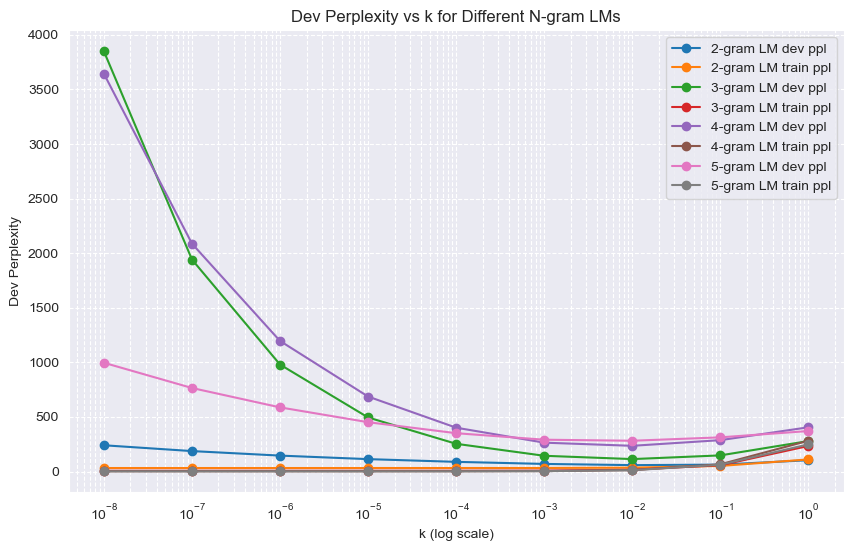
\includegraphics[width=0.8\textwidth]{ppls.png}
            \caption{Perplexities of different n-gram models}
            \label{fig:perplexities}
        \end{figure}
        The best model is seen to be the 2-gram model with learning rate 0.01.


        \item For interpolation, I get:
        \begin{figure}[H]
            \centering
            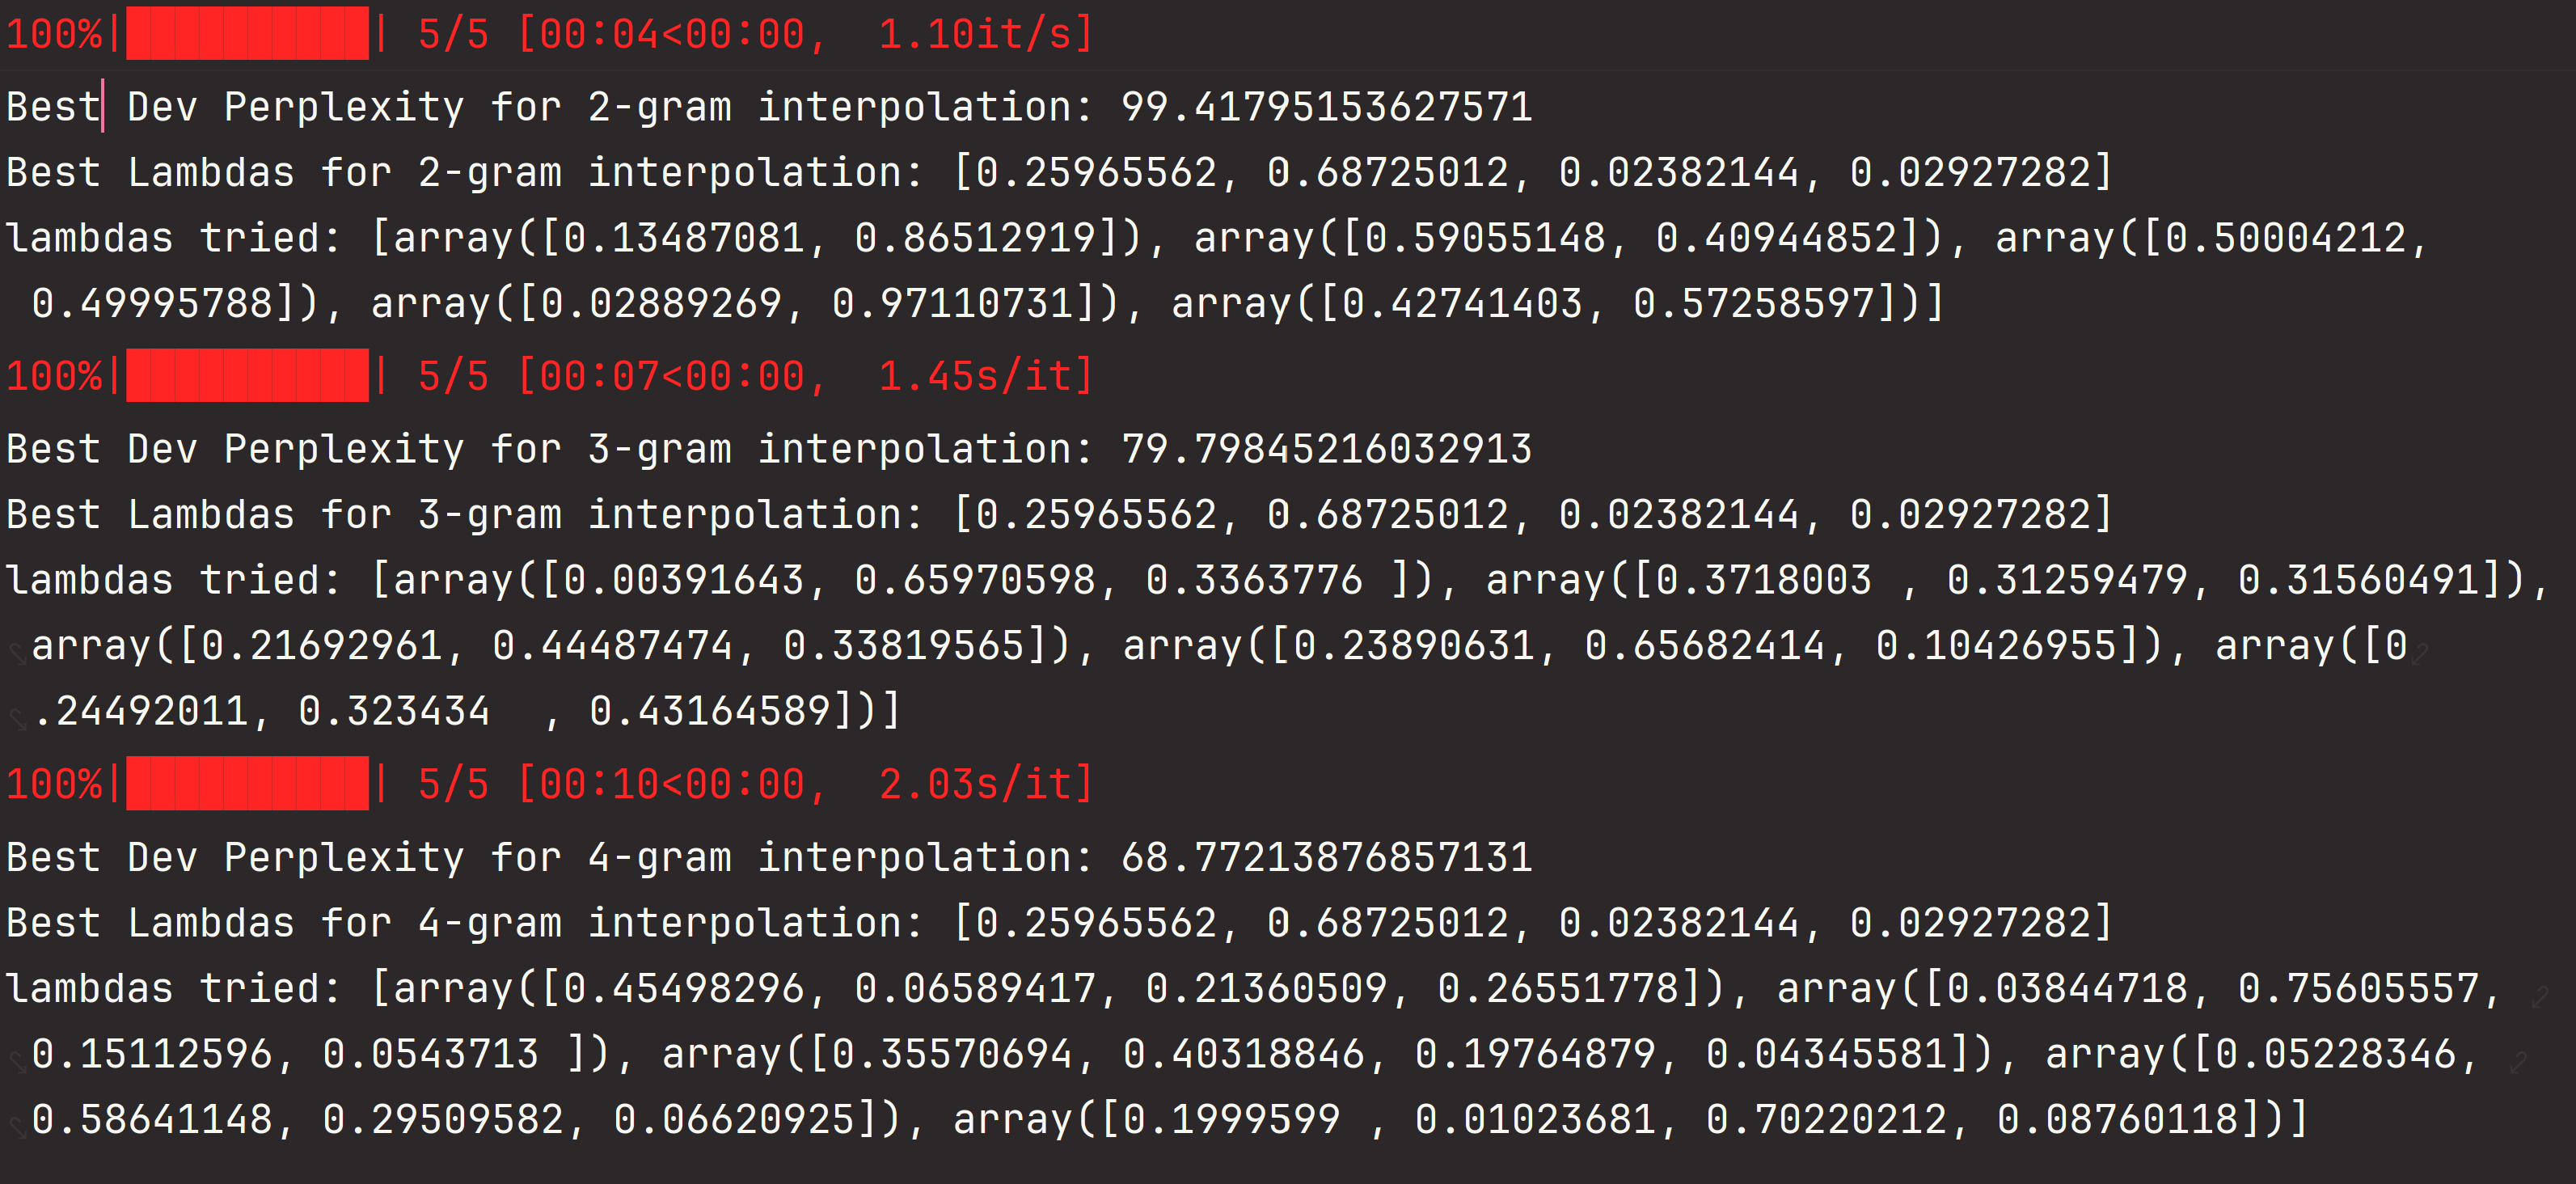
\includegraphics[width=0.8\textwidth]{interpolationppls.png}
            \caption{Perplexities of different n-gram models with interpolation}
            \label{fig:interpolation_perplexities}
        \end{figure}
        I sampled the $\lambda$s from the Direchlet distribution, which is a uniform distribution for the $\lambda$s that sum to 1. 
    \end{enumerate}
    
\end{document}